\chapter{Explaining Neural Networks}

% This section covers intro to explainablity of neural networks.
% We define aims and scope of explainability
% Why do we want to be able to explain models.
% some legal criterions
% some paper about patholigists not really believing the network. 
% We discuss utilized methods.

This chapter covers introduction to the growing field of explainable artificial intelligence. We start with short overview of the field itself, following by motivation for understanding decision of neural networks, alongside overview of legal obligations placed on decision support systems by European Union. We continue with overview of several explainability methods, suitable for our domain and task. This will serve as a foundation for the next chapter, where we evaluate selected methods against our benchmark.

In the contemporary literature, several terms are used when addressing the incomprehensibility of ML models. Arrieta et al. distinguish following idioms []:
% TODO - make actual definitions

\begin{enumerate}
    \item Understandability: Characteristic of a model to make a human understand its function without any need for explaining its internal structure or the algorithmic means by which the model processes data internally
    \item Comprehensibility: Ability of a learning algorithm to represent its learned knowledge in a human understandable fashion 
    \item Interpretability: Ability to explain or to provide the meaning in understandable terms to a human.
    \item Explainability: An accurate proxy of the decision maker and comprehensible to humans.
    \item Transparency: A model is considered to be transparent if by itself it is understandable.
\end{enumerate}

They further emphasize the distinction between interpretability and explainability -- interpretability, closely coupled with transparency are inherent and passive characteristics of a machine learning model. On the contrary, explainability is an initiated action taken to clarify model's internal details . Both can be seen as means to achieve understandability -- how a human can make senso of decisions made by the model [].

% https://pdf.sciencedirectassets.com/272144/1-s2.0-S1566253519X0007X/1-s2.0-S1566253519308103/main.pdf

\section{Need for understandability}

State of the art neural network models are often products of billions of parameters []. A term "black-box" models has been coined, to highlight their complex internal mechanics. In a crusade for ever-better performance and accuracy, models inherently grow in size and depth. Increasing size and complexity raises concerns of research community and general public, whether these networks can be trusted and used responsibly. [] []

% https://pdf.sciencedirectassets.com/272144/1-s2.0-S1566253519X0007X/1-s2.0-S1566253519308103/main.pdf
% https://ieeexplore.ieee.org/document/8400040

\subsection{Spurious Correlations}
% systematic bias & reserch
Distrust does not stem only from lack of insight into model's internal reasoning. In certain cases, seemingly flawless performance of machine learning models may in fact be a result of a systematic bias in training and evaluation data. Commonly used example is an experiment by Ribeiro et al. where they purposely trained a logistic regression classifier to distinguish between wolves and husky dogs. The training dataset was arranged, such that wolf pictures have snow in their background and the husky counterpart does not. This led the classifier to make its decision based on the presence of snow in the picture, rather of the animal []. 

% husky - https://arxiv.org/pdf/1602.04938.pdf

Another, less artificial example is shown in Figure \ref{fig:horse-tag}. One can see, that a \emph{capable} model may produce a desired output, despite that the presence of features important for a human decision in input data had no influence on model's decision.

Instances such as these demonstrate that the understandability of a decision support system isn't just an issue for the end-user. It's also advantageous for the model's development cycle. Gaining insights into the factors influencing the model's decisions allows us to responsibly evaluate if its reasoning aligns with our expectations -- and take according measures if not.


\begin{figure}[!h]
    \begin{center}
    \begin{minipage}{1\textwidth}
      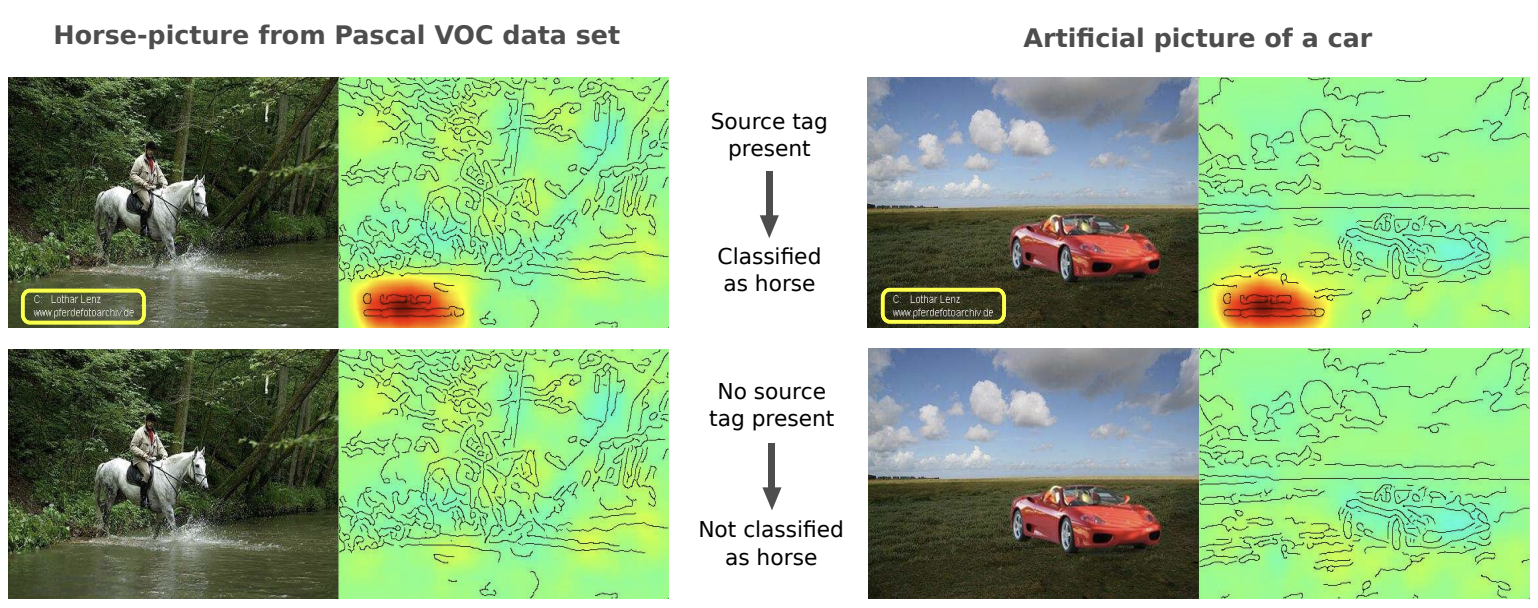
\includegraphics[width=\textwidth]{img/horse-tag.png}
    \end{minipage}
    \caption{Experiment conducted by Samek et al []. Model was trained on PASCAL-VOC dataset []. After the training, they found presence of so-called \emph{spurious correlation}. Pictures of horses are classified solely on whether the bottom-left corner of an input image contains a source tag. If the source tag manually added to an otherwise correctly classified image of a car -- the model changes its prediction, and the image is classified as a horse instead.}
    \label{fig:horse-tag}
    \end{center}

\end{figure}

% horse - https://arxiv.org/pdf/1902.10178.pdf

% medicine pov
\subsection{Explainability in medical domain}

Such spurious correlations and the black-box tag lead clinicians to be sceptic about integrating AI in healthcare. Recent survey by GE HealthCare concludes, that out of 2000 clinicians participating in the survey, $58$ percent does not have overall trust in AI systems and $44$ percent of respondents believe, that the AI-based systems are biased []. Achieving trust of both clinicians and patients is crucial in order to achieve industry-wide utilization of machine learning-based systems.

% https://www.gehealthcare.com/about/newsroom/press-releases/ge-healthcare-reimagining-better-health-study-identifies-the-barriers-to-achieving-a-more-human-and-flexible-healthcare-experience



% legal
\subsection{Legal obligations for AI explainability in the European Union}

Given certain applications, understanding the model is not only a moral obligation.

In 2016, the European Union included what is often referred to as the "right to explanation" within the General Data Protection Regulation (GDPR). Specifically, Articles 13 and 14 give individuals the right to receive "meaningful information about the logic involved", when they are a part of automatic decision process making.  This pose a challenge for industry, implicating that adequate measures need to be taken in place in order to fully integrate decision support systems based on deep learning. More on what Articles 13 and 14 mean for AI is to be found in a paper by Goodman and Flaxman [].

% https://arxiv.org/pdf/1606.08813.pdf

Another piece of legislation from the European Union is anticipated to be implemented in May or June of 2024. \emph{AI Act} introduces a series of regulations for machine learning-based AI systems. The legislation is notably more detailed and exhaustive than Articles 13 and 14 of the GDPR, yielding mixed responses from domain experts. While the full implications are yet to be seen, it already imposes several restrictions on what needs to be met before deploying machine learning models. In particular, one section specifically targets high risk AI systems and that a "Providers must build for human oversight, incorporating ‘human-machine interface tools’ to ensure systems ‘can be effectively overseen by natural persons’". Several other important aspects of model's lifecycle are revised as well, ranging from training dataset to technical documentation. Comprehensive overview of the article is beyond the scope of this thesis, and is summarized by Veale and Borgesius in [].

% https://www.degruyter.com/document/doi/10.9785/cri-2021-220402/html

\section{Explainable Artificial Intelligence}

Rapid development of deep learning models and scarcity of trust among users call for tools and methods, which allow us to understand and justify outputs of otherwise opaque systems. With the aim to shed light on internal processes of machine learning models, a sub-field of Explainable Artificial Intelligence (XAI) covers a range of techniques to make models more explainable, while preserving their performance and effectiveness. XAI techniques enable humans to build trust and manage machine learning based decision support systems -- a crucial part of assimilation of systems based on deep learning [].

\todo{find citation, forgot to write down}

The exact borders of the field are not firmly set, and the notion of what does it mean to explain a model is an ongoing matter of discussion. 

Throughout this thesis, 'XAI' will refer specifically to the subfield dedicated to advancing explainability in AI, while 'explainable artificial intelligence' will denote the attribute of machine learning models that enables certain level of understandability.


\subsection{How do we achieve explainable artificial intelligence?}

\emph{Unfortunately, “explainability” is a nebulous and elusive concept that is hard to target.} []
\newline
% https://arxiv.org/pdf/2209.00366.pdf

In order to achieve something, it is important define the scope. To describe explainable artificial intelligence, Arietta et al. [] suggest to use following definition: \emph{Given an audience, an explainable Artificial Intelligence is one that produces details or reasons to make its functioning clear or easy to understand}.
% taxonomy paper

We distinguish between following two means, how to make artificial intelligence understandable:

\begin{enumerate}
    \item Transparent model: Models based on linear regression or decision trees are inherently interpretable -- therefore understandable by itself. By looking at their parameters, we are able to clearly derive, how they came to given conclusion.
    \item Post-hoc explainability methods: When dealing with e.g. neural networks, we gain little insight into how they operate by simply inspecting their weights. Therefore we must implement auxiliary methods, which simplify and distill the reasoning of networks, so that according to the definition -- we get a clear and easy to understand explanation. Post-hoc explainability methods can be further divided into two subgroups -- global methods explaining model as a whole and local methods, focused on internal reasoning behind prediction for particular input sample.
\end{enumerate}

In the recent years, plethora of both global and local post-hoc explainability methods has been introduced in order to help grasp decision process of deep neural networks []. Post-hoc methods can be further divided into two groups: 

\begin{enumerate}
    \item Model-specific methods: designed to explain only models with specific features and capabilities -- such as attention-based models or convolutional neural networks.
    \item Model-agnostic methods: can be used to explain arbitrary machine learning model.
\end{enumerate}

% https://pdf.sciencedirectassets.com/272144/1-s2.0-S1566253519X0007X/1-s2.0-S1566253519308103/main.pdf

As of now, there is no universal guideline on how to choose the correct explainability method, and the choice needs to be adapted according to ones domain needs. We need to keep in mind several factors when choosing a suitable method. In definition of explainable artificial intelligence we use in this thesis, authors put emphasis on the \emph{audience} of the generated explanations.

Given a model, end user verifying trustworthiness and fairness of the result and researcher trying to debug the model are likely to demand different forms of produced explanations. Additionally, performance and complexity of the method itself are all important factors, which we need to consider when determining which method to use.

% we can cite the Arrieta paper here, but I came up with this on my own.

\subsection{Explaining RationAI's model with Occlusion}

To achieve goal of this thesis and find suitable method, we are not starting from square one. There has been efforts to find a suitable method. RationAI's team partially succeeded, by utilizing explanation based on occlusion based saliency.

\subsection{Occlusion}

Current post-hoc method employed to explain decisions of model described in Section X is occlusion-based saliency. Occlusion is model-agnostic method and comes from family of so-called input perturbation based methods. Occlusion generates attribution map by systematically covering square parts in input image and observing the change in models prediction confidence on the perturbed image. On intuitive level, we expect that when we cover (occlude) important part of input image, the confidence of our classifier drops. In contrary, when we cover region which does not contain any important features, the output should not differ too much from output for the original pixel.

Experiment conducted by Gallo et al. [] shows, that in the setting of prostate cancer detection, the method produces semantically correct explanation maps. Sadly, occlusion comes with high computational complexity and resource utilization. For our use-case, explaining a single tile of $512px \times 512px$, the method needs 289 forward passes to compute the attribution map. In production setting, on a machine with 8 cores, 16GB of RAM and 48GB of GPU memory capacity, occlusion needs approx. 2 seconds and 40GB of GPU memory to generate single heatmap. Recall Section Y and processing WSI. In our test set, slide size varies from 400 to 4000 tiles per slide. Ommiting auxiliary attribution map processing, this method takes  
% https://pdf.sciencedirectassets.com/277035/1-s2.0-S1871678423X00065/1-s2.0-S1871678423000511/main.pdf


In the production settings, size of the occlusion patch is 55 x 55 px and stride is set to 27 px. With those parameters in place, we need 289 forward passes through our our model to explain one patch. With production system resources, this solution takes about 2 seconds and approx. 40GB of GPU memory to compute attribution map for a single image. Recall, that number of patches of WSI's from test set is ranging from 400 to 4000.



\section{Operation Tenebris: Candidate Explainability Methods} % working name, not real

% here i want to introduce, how we select methods - literature is unclear. But we have a set goal and existing solutions -- therefore we will look for methods which produce the output in the given form -- as local attribution map
%sal

In this section we overview current solutions and other explainability methods we will compare against current solution. When choosing methods, we kept several deciding factors in mind:
% attribution map vs saliency map

\begin{enumerate}
    \item Explanation form: The current solution produces attribution heatmaps, and we do not want to change that. Our domain expert is used to work with them and they fit perfectly for our use case.
    \item Availability: We do not aim to implement methods by ourselves -- there are several widely used machine learning libraries supporting wide array of methods. In this thesis, we used libraries \emph{captum}, \emph{pytorch-grad-cam} and \emph{zennit}. 
    \item Internal Mechanism: Methods utilize different principes when computing respective attribution heatmaps. Perturbation based methods usually require several forward passes to compute single heatmap -- rendering them slower in general. On the other hand, gradient or redistribution based methods usually rely only on one pass, making them more suitable to achieve our initial goal of speeding everything up.
\end{enumerate}

During this section, when referring to a model, we mean model employed by RationAI introduced in Section TBD.

\todo{ref section}

\subsection{GradCAM++}

\subsection{HiResCAM}

\subsection{ScoreCAM}

\subsection{AblationCAM}

\subsection{Layerwise Relevance Propagation}